\section{Dokumentengeschichte}
\begin{table}[h]
 \begin{tabular}{|l|l|p{4cm}|}
 \hline
 Zeitraum & PL/Autor(en) & Änderungen \\
 \hline
 Sommersemester 1980 & IHR NAME & 
text \newline 
text \newline 
text \newline 
text \newline 
text \newline 
text \newline 
 
  \\
 \hline
 Wintersemester 2017/18 & Behzad Karimi & 
Bild eingefügt (Bilder ab jetzt mit 120mm einfügen) \newline 
text \newline 
text \newline 
text \newline 
text \newline 
text \newline 
 
  \\
 \hline
 \end{tabular}
 \caption{Dokumentengeschichte}
 \end{table}

\section{Aufgabe der Komponente}
\begin{figure}[h!]
\centering
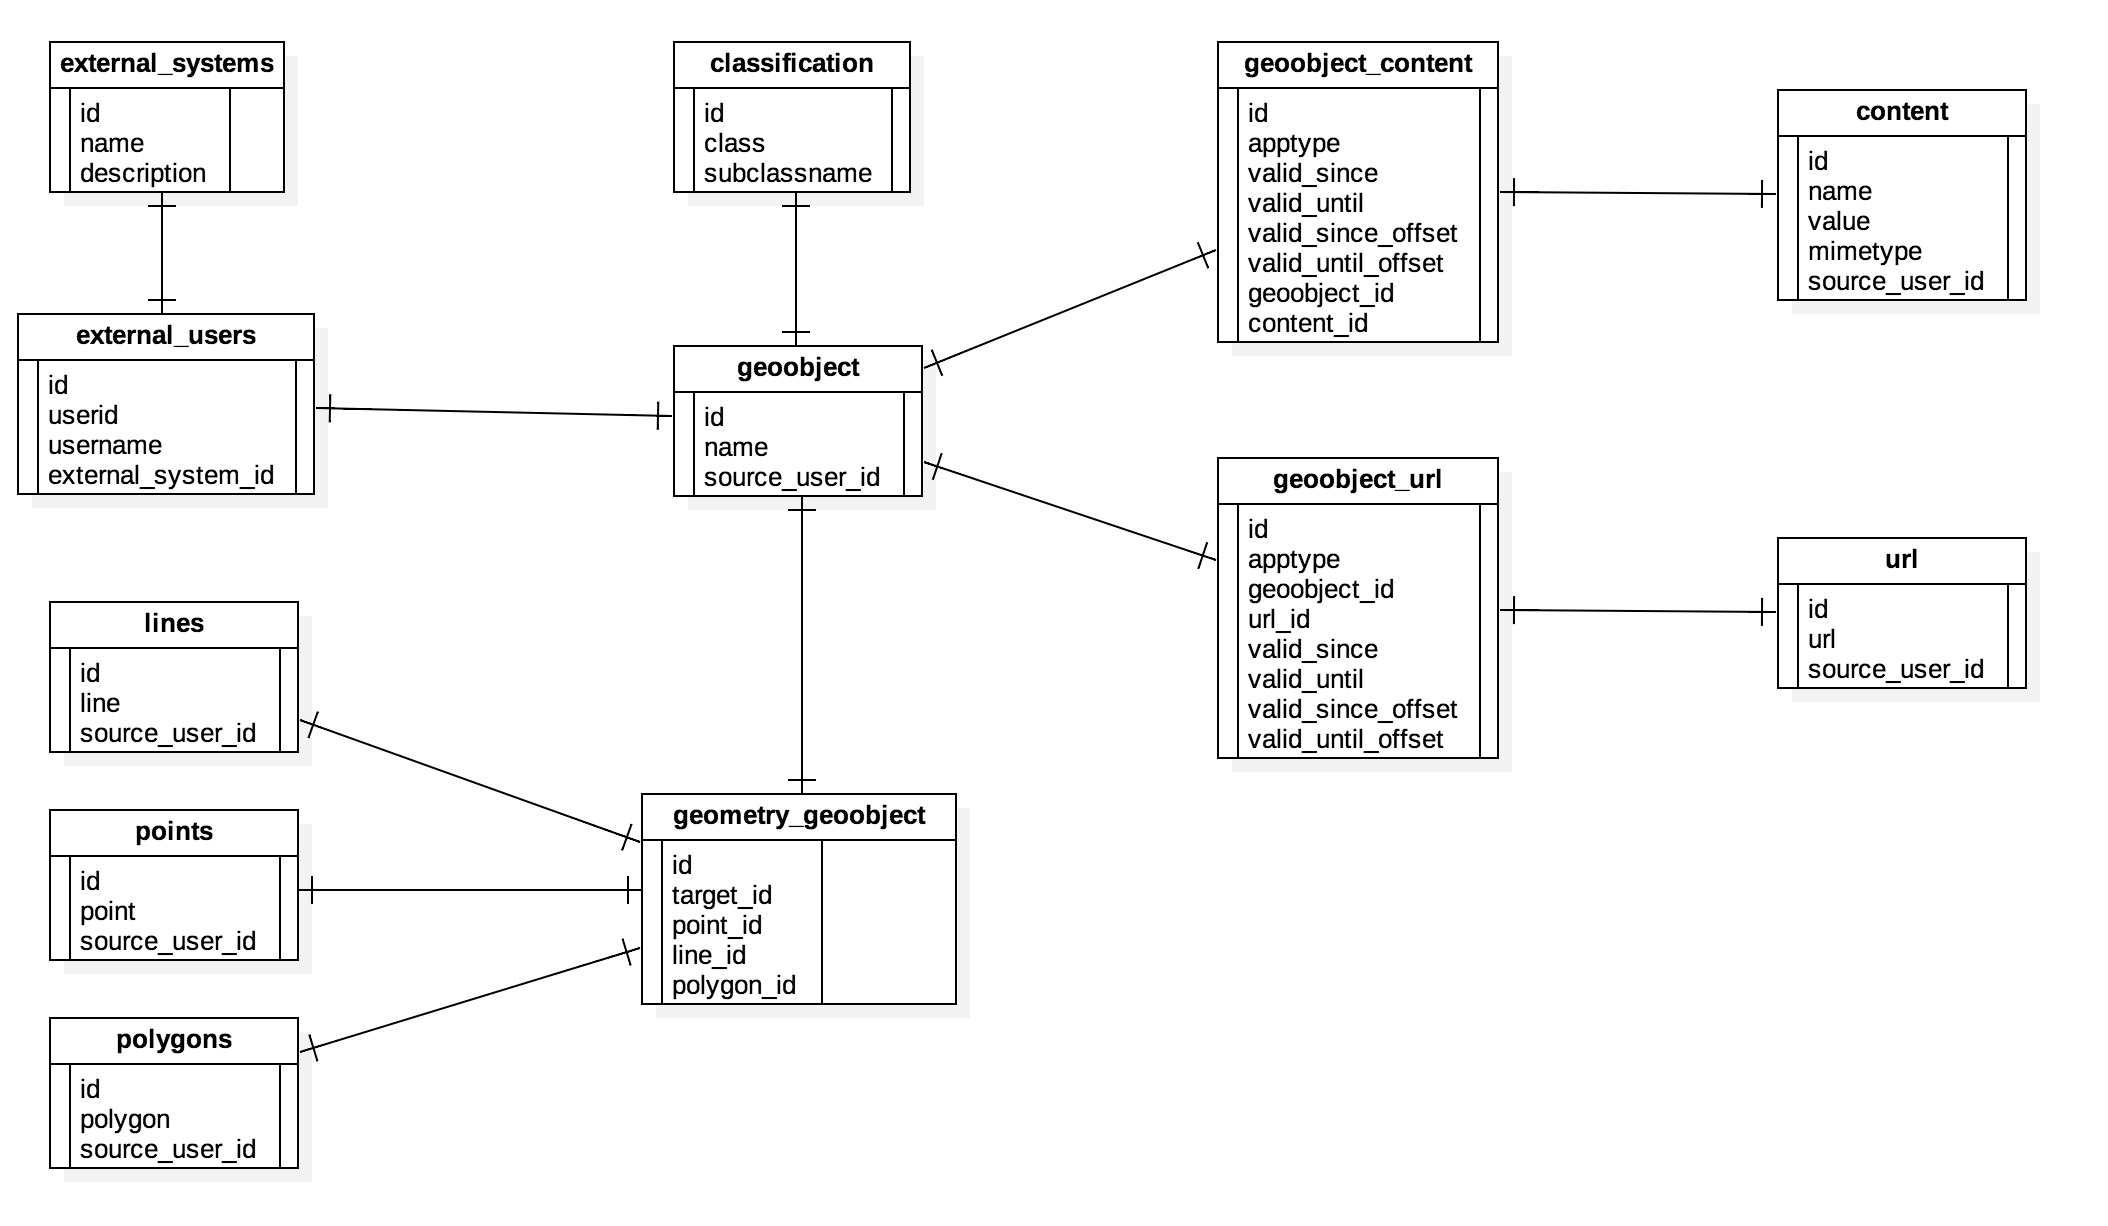
\includegraphics[width=120mm]{ohdm_datenmodell/ohdm_data_modell.jpg}
\caption{OHDM Datamodell}
\label{fig:datamodell}
\end{figure}
Das Datenmodell von OHDM ist recht simpel. Wie an der \cref{fig:datamodell}.
Verbale kurze prägnante Beschreibung, was die Komponente leisten soll.
Das sind wenige Seiten.

(Ausfüllen in Prototyp-Phase)

\section{Architektur}

\subsection{Überlick}
Grafik der Teile der Komponente (wichtig: Benennung aller Schnittstellen). 
Anwendung der Komponente nennen (Use Case).

Übliche Interaktionen durch Interaktionsdiagramme.

(Ausfüllen in Prototyp-Phase)

\subsection{Schnittstellendefinitionen}
Beschreibung der angebotenen Schnittstellen. Benennung der Funktionen
mit Vor- und Nachbedingungen. Beschreibuung des Protocol-Bindings.

(Beginnen in Prototyp-Phase. Konkretisieren in der Alphaphase)

\subsection{genutztes Komponenten}
Beschreibung, welche weiteren Komponenten (in welchen Versionen, wo beziehbar) genutzt werden.

(Beginnen in Prototyp-Phase. Konkretisieren in der Alphaphase)

\section{Nutzung}
\subsection{Code}
Wo findet man den Code. Struktur des Codes. (In Prototyphase ausfüllen,
kann dort sehr kurz sein. Ab Alpha-Phase konkret beschreiben.)

\subsection{Deployment / Runtime}
Beschreibung wie die Komponenten aus dem Quellcode erzeugt werden kann,
wie sie installiert wird und wie man sie startet.

\section{Qualitätssicherung}
(Ausfüllen ab Alpha-Phase).

Wie erfolgt die Sicherung der Qualität? Keine Romane, sondern ehrlich notieren,
was man tut. Wenn man nichts tut, dann steht hier: Wir sichern die Qualität der
Komponente nicht.

Issue-Tracking: wie erfolgt das, interne Fehlermeldungen (ab Alpha), 
externe Fehlermeldungen ab Beta.

\subsection{Test}
Wie wird die Komponente getestet.

\section{Vorschläge / Ausblick}
Was ist aufgefallen, was sollte man ändern? Löschen Sie auch gern die Kommentare
der Vorgänger, aber nur, wenn es wirklich nicht mehr relevant ist.

